\section{Functionality Testing}
\label{sec:functionality-testing}

Following the functionality testing methodology defined in Section \ref{subsec:functionality-testing-plan}, that assesses core Functional and Non-Functional requirements of the \ac{grs} and \ac{acc},
the following was conducted:

\paragraph{FT1 --- Identity Registration}
The \ac{grs} and \ac{acc} applications were started, with the connected camera --- a Logitech C920 HD Pro Webcam --- set up on a tripod facing a blank wall (for contrast).
Figure \ref{fig:system-testing-hardware-setup} below shows an example setup of the camera and tripod facing a blank wall. 

\begin{figure}[H]
	\centering
	\begin{minipage}[t]{0.48\textwidth}
		\centering
		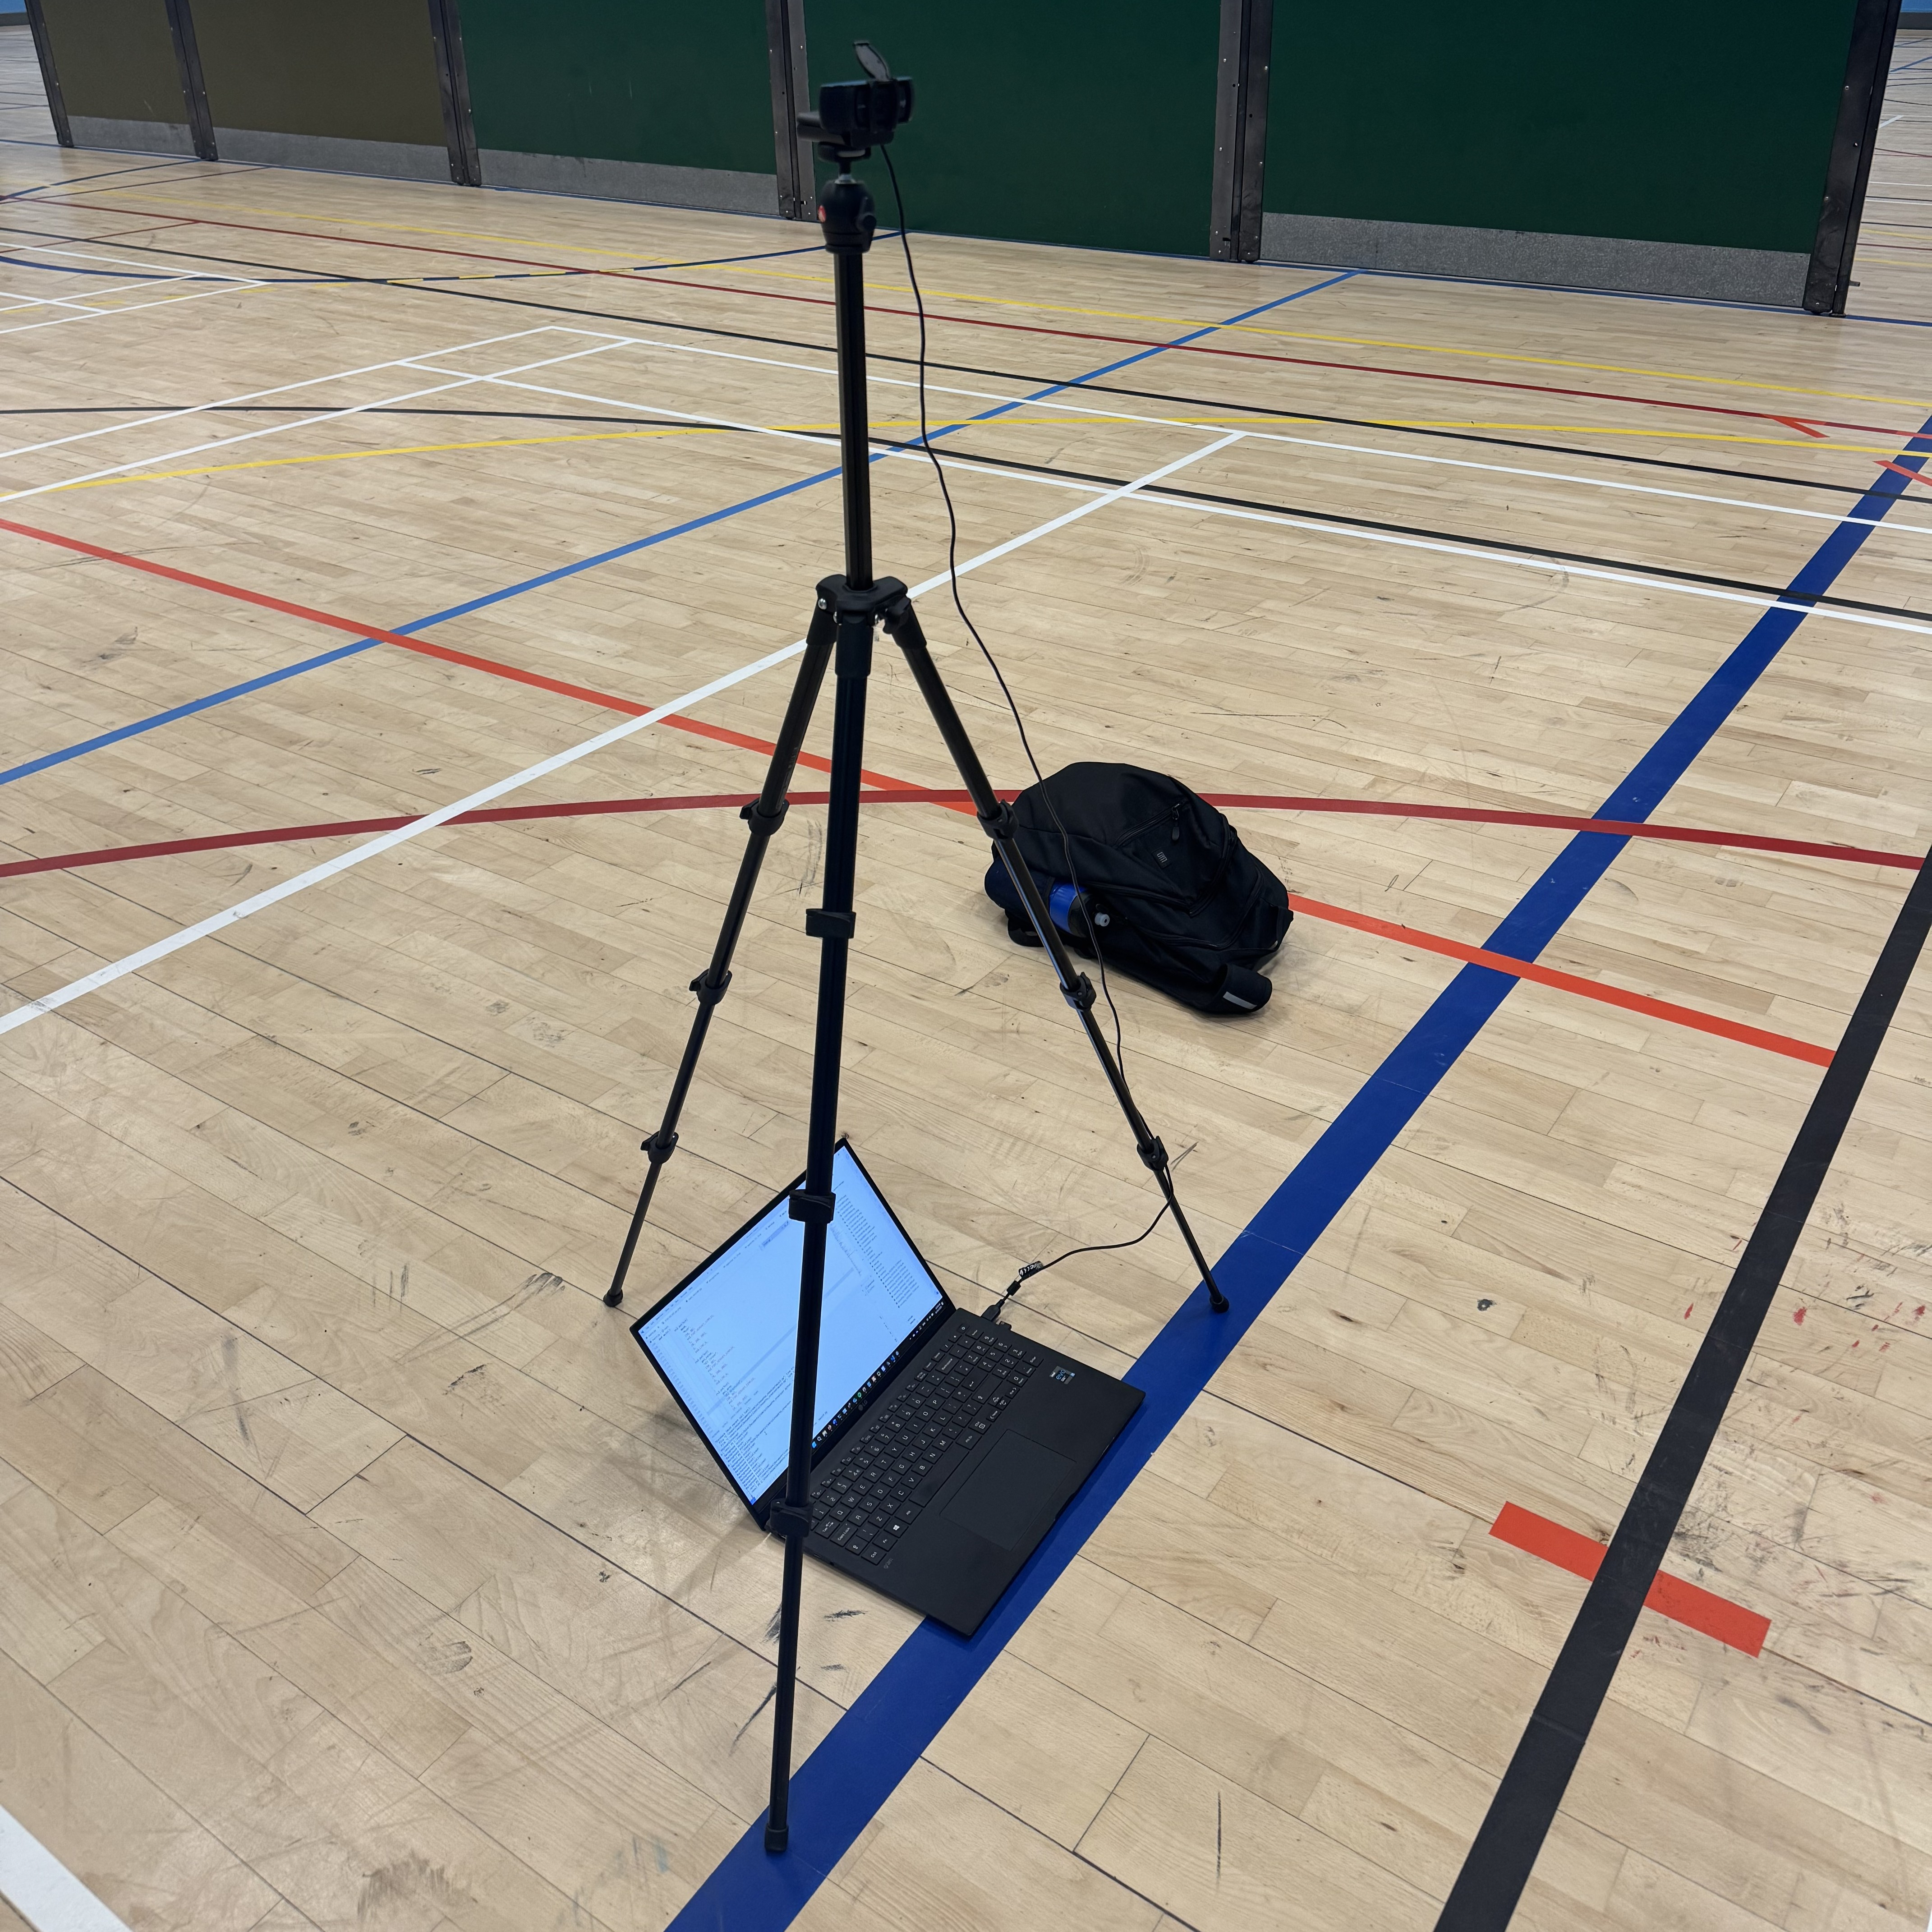
\includegraphics[width=\textwidth]{assets/hardware-setup_1.JPEG}
	\end{minipage}\hfill
	\begin{minipage}[t]{0.48\textwidth}
		\centering
		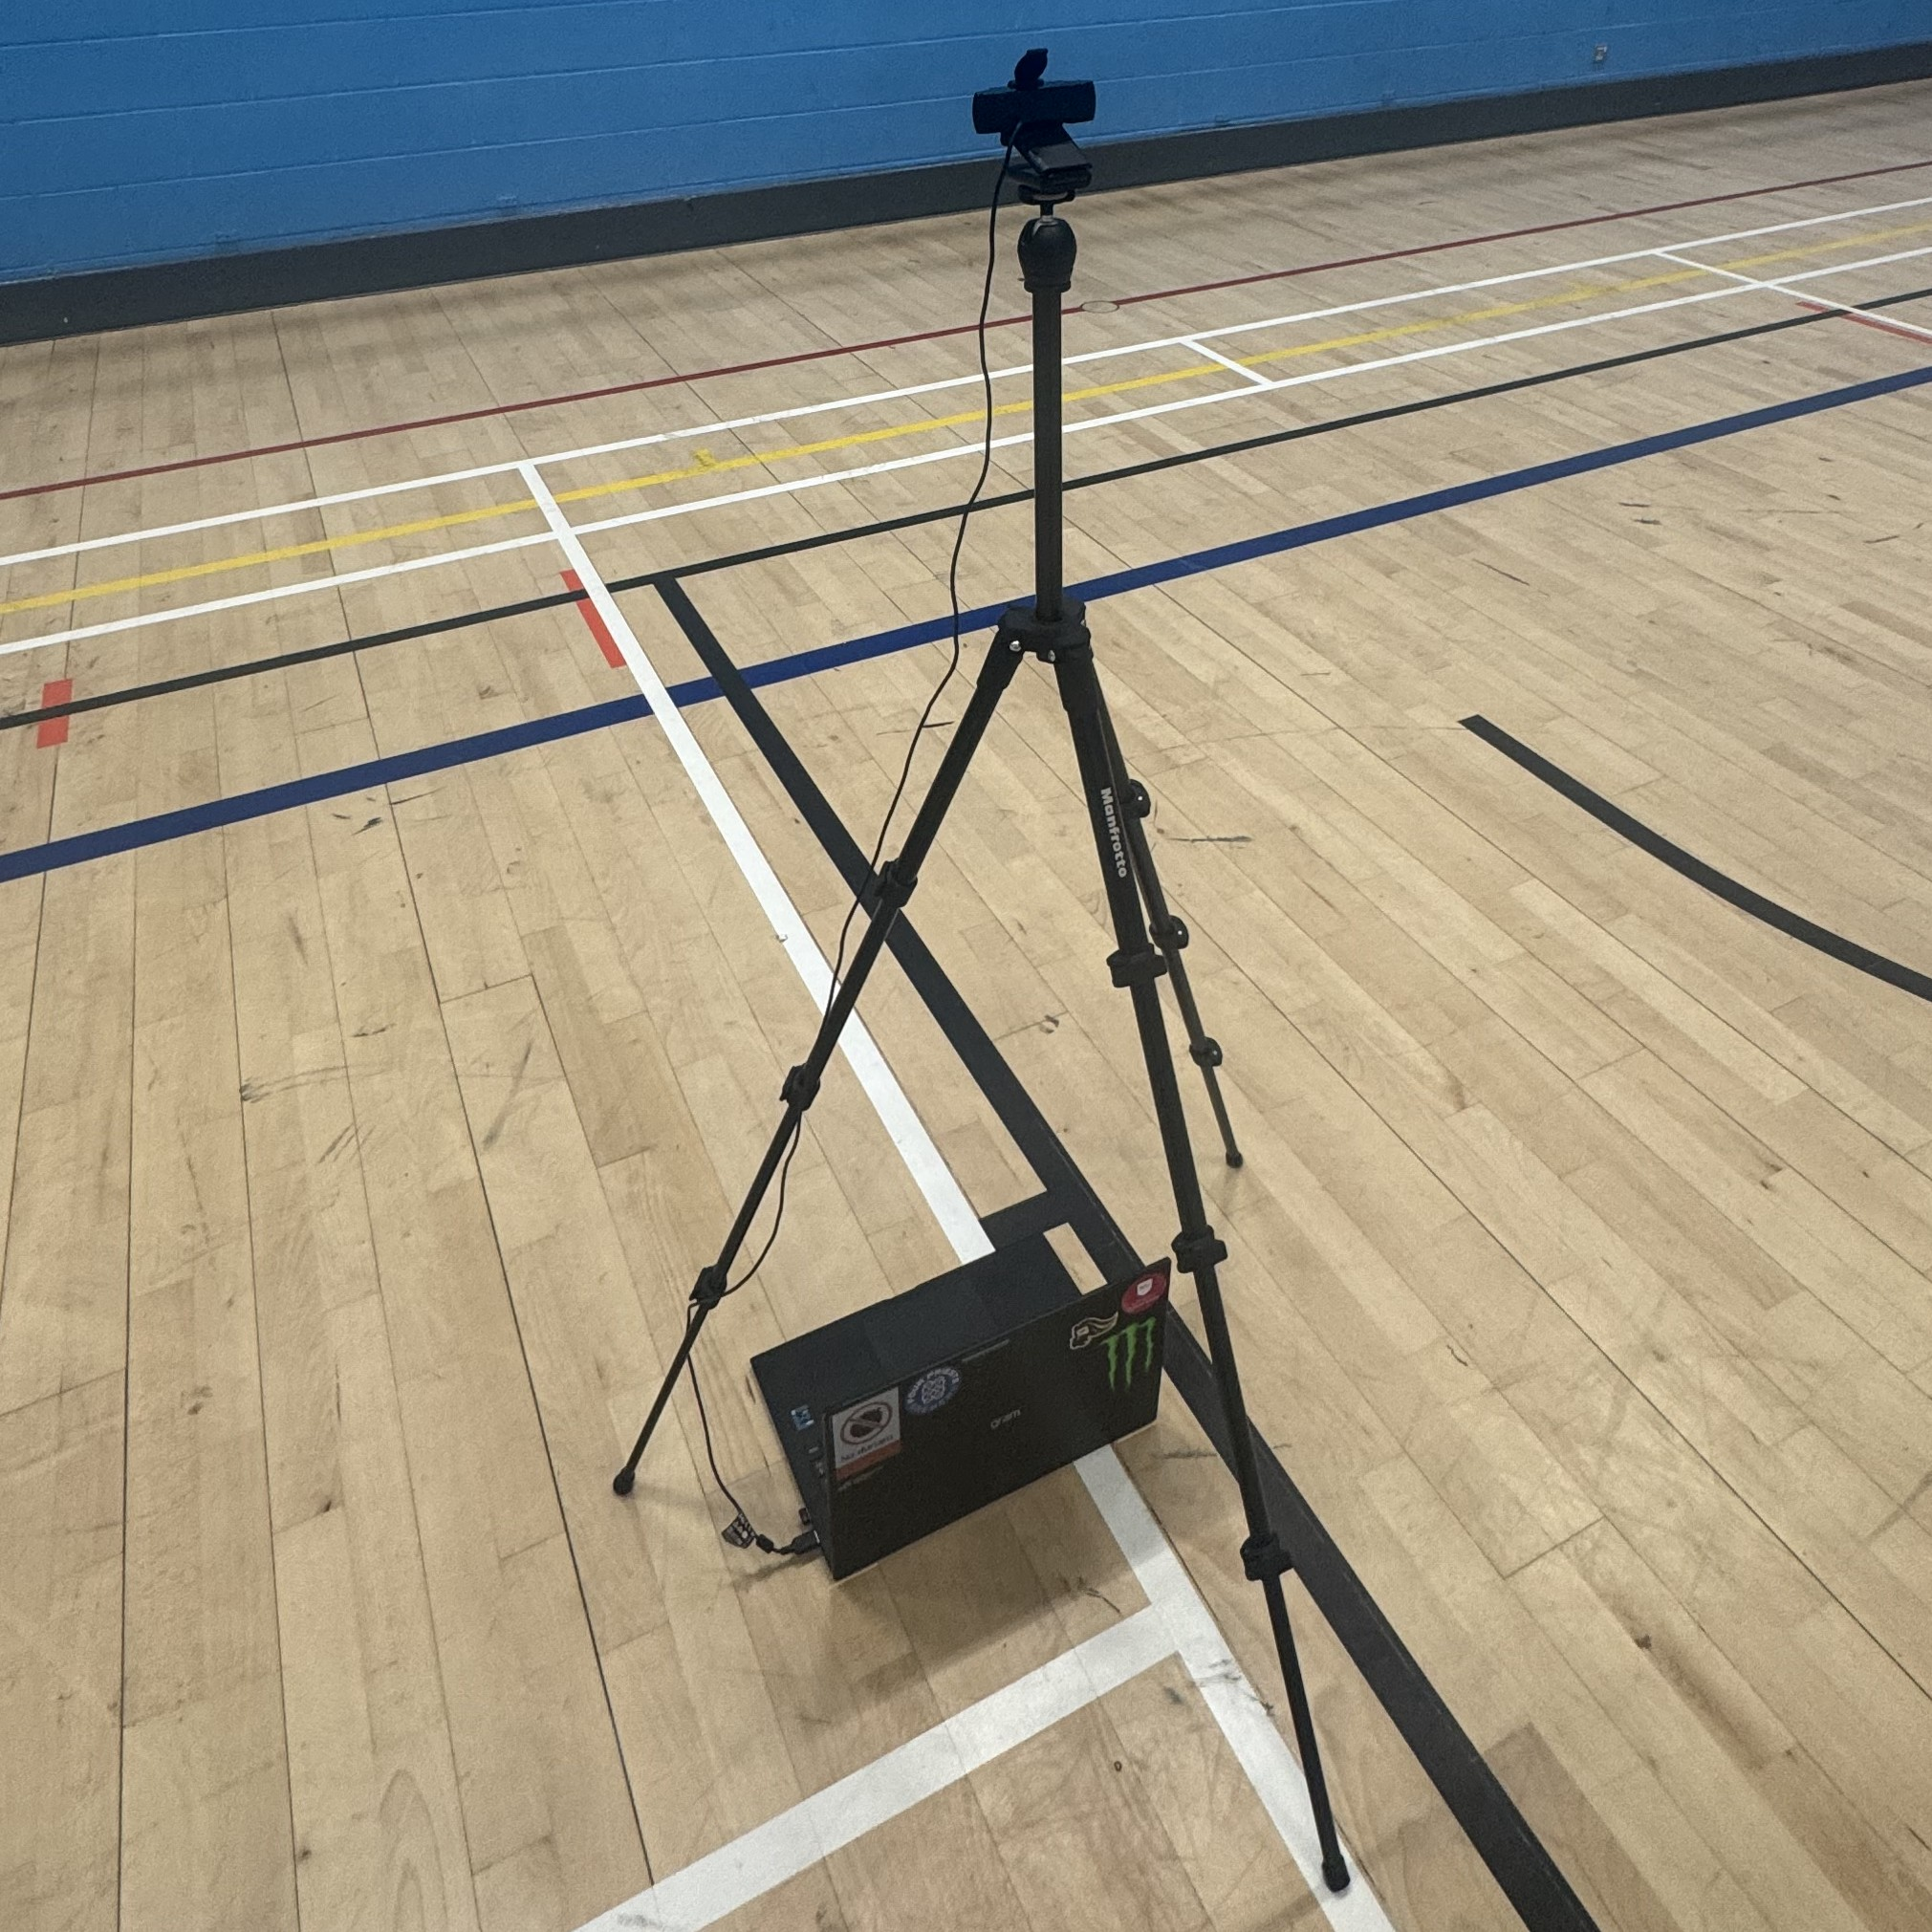
\includegraphics[width=\textwidth]{assets/hardware-setup_2.JPEG}
	\end{minipage}
	\caption{System Testing Hardware Setup}
	\label{fig:system-testing-hardware-setup}
\end{figure}

Following software initialisation and hardware setup, a subject walked in a straight line through the camera's field of view, from three meters away (ensuring the entire subject was within frame).
The subject was instructed to walk at a normal pace, and was asked to stop after three seconds.
Figure \ref{fig:identity-registration-walk} below shows the resulting \ac{gei} preview displayed in the \ac{acc} \ac{ui} after the subject (this has been substituted for the report author to protect confidentiality of volunteer biometrics) had exited the frame.

\begin{figure}[H]
	\centering
	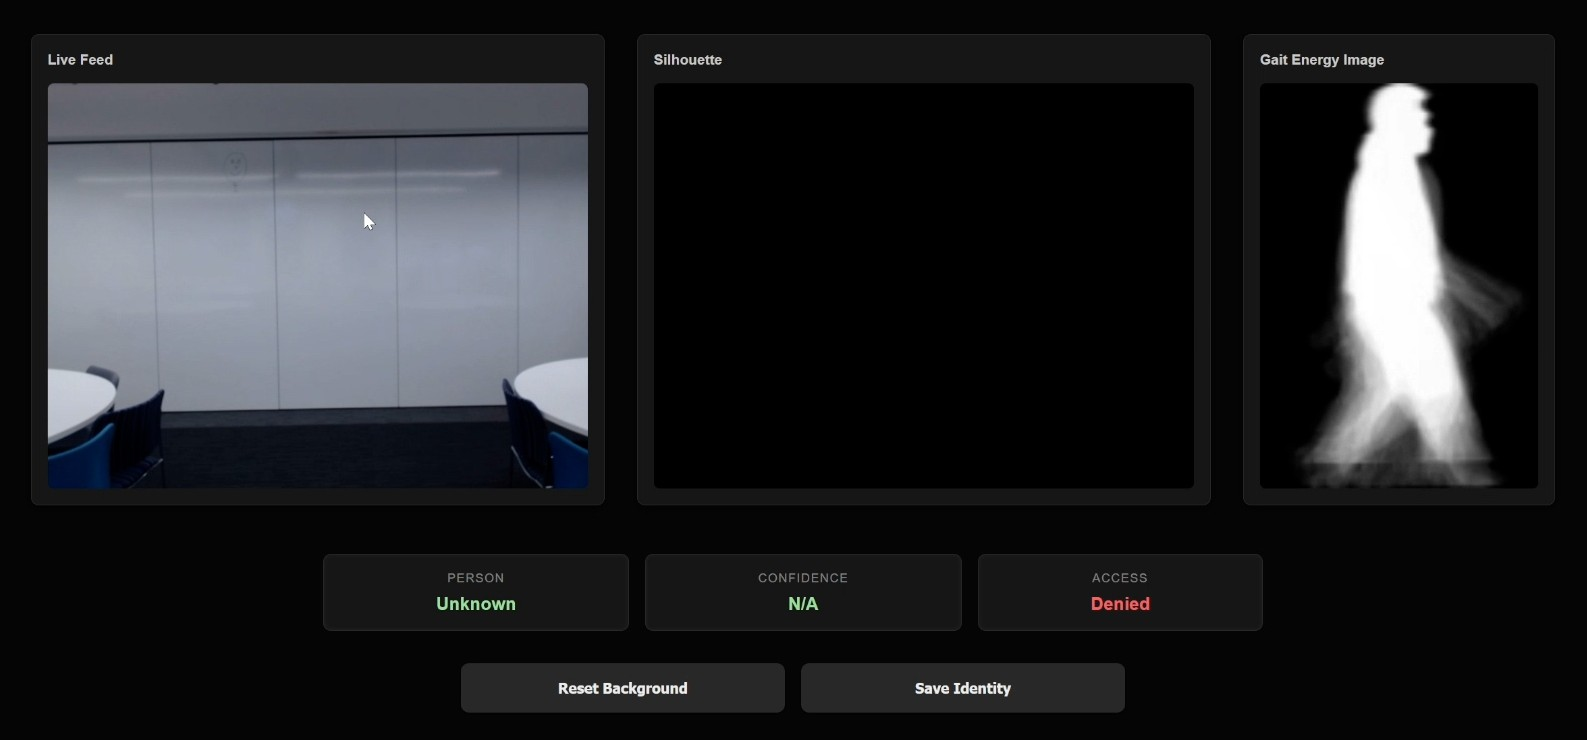
\includegraphics[width=0.8\textwidth]{assets/post-cycle.jpg}
	\caption{Post-Cycle-Capture \ac{gei} Preview}
	\label{fig:identity-registration-walk}
\end{figure}

After the subject had exited the frame, the 'Save Identity' button was clicked, a label was entered, and the \ac{acc} application submitted the combination of the \ac{gei} and label to the \ac{grs}' \codeword{/api/register} endpoint.

The \ac{grs} \ac{ui} was then refreshed, with the new registered identity displayed in the 'Registered Identities' grid, with the subject's label, ID number, and \ac{gei} preview image --- shown in Figure \ref{fig:identity-registration-gei} below.

\begin{figure}[H]
	\centering
	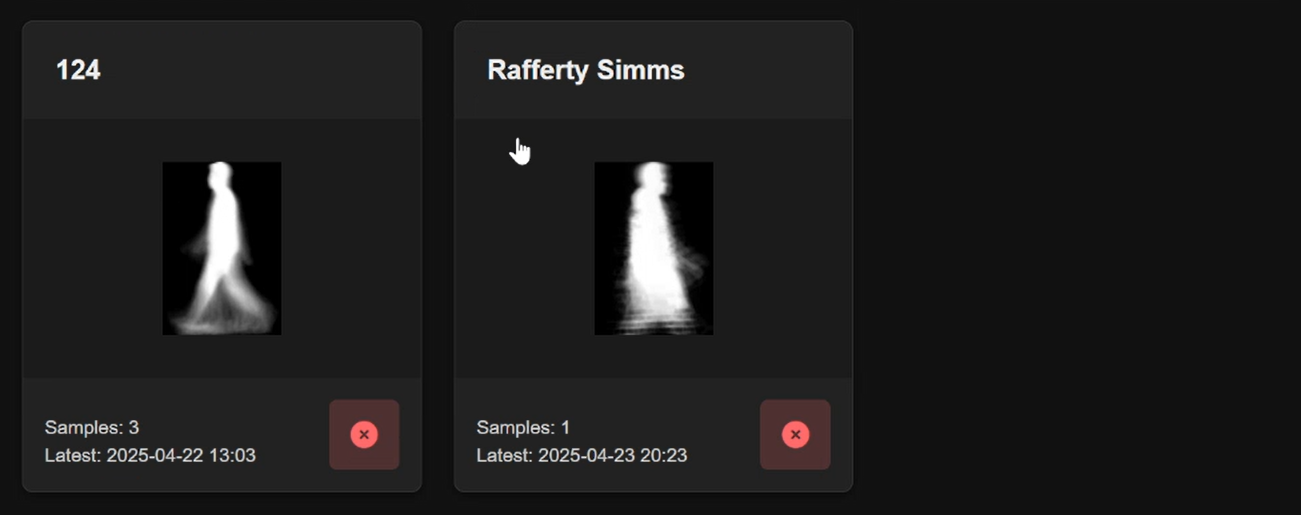
\includegraphics[width=0.8\textwidth]{assets/added-identity.png}
	\caption{New Identity Added to Registered Identities Grid}
	\label{fig:identity-registration-gei}
\end{figure}

\begin{adjustwidth}{1cm}{}
	\begin{tcolorbox}[
		boxrule=0pt,
		skin=bicolor,
		colback=green!5,
		colbacklower=red!5,
		frame empty,
		borderline={0pt}{0pt}{white}, % removes potential inner borders
	]
	This result aligns with what was expected for\#FT1, with users able to capture gait cycles, producing a \ac{gei}, which can then be saved to the \ac{grs} database.
	This is a core requirement for this project as a whole.
	
	\tcblower
	
	\paragraph{Issues} Testing of gait cycle capture and \ac{gei} creation was not smooth sailing. Although generally sucessful, results suffered when the background was low contrast to the subject (e.g., a dark background and dark clothing).
	This would result in areas of the silhouette being misidentified as background, and therefore being excluded from the silhouettes and resulting \acp{gei}.
	\end{tcolorbox}
	
\end{adjustwidth}


\paragraph{FT2 --- Identity Removal}
The identity registered in \#FT1 and displayed in the 'Registered Identities' grid was selected, loading its 'Identity' page.
The delete button in the top right corner of the page was then clicked, displaying a confirmation dialog shown in Figure \ref{fig:identity-removal-confirmation} below.

\begin{figure}[H]
	\centering
	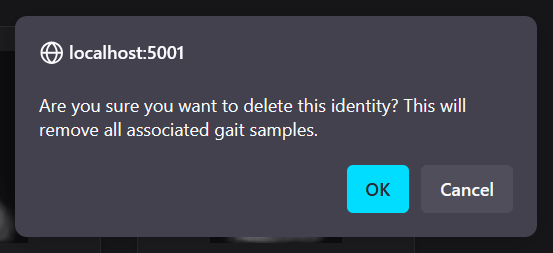
\includegraphics[width=0.65\textwidth]{assets/delete-confirmation.png}
	\caption{Identity Removal Confirmation Dialog}
	\label{fig:identity-removal-confirmation}
\end{figure}

The 'OK' button was then clicked, removing the identity from the database along with any associated \ac{gei} samples and access control rules, with the \ac{grs} \ac{ui} redirecting to the home page where the grid of registered identities was empty --- as expected.

\begin{adjustwidth}{1cm}{}
	\begin{tcolorbox}[colback=green!5, boxrule=0pt, frame empty]
		This result aligns with what was expected for \#FT2, with the identity and all associated data removed from the \ac{grs} database.
		This is a critical requirement for systems handling sensitive (biometric) data, ensuring legislations such as the \ac{gdpr} are adhered to.
	\end{tcolorbox}
\end{adjustwidth}

\paragraph{FT3 --- Identity Classification of Known Subject}
Due to the prediction-based nature of the \ac{grs}' classification model, testing the efficacy of the system required a number of samples to be captured and registered before this test could be conducted.

Five (5) identities were registered (using volunteers from the University's student population), with one (1) sample captured for each subject.
\textit{Note: Data was stored under anonymised labels to ensure confidentiality and was deleted after testing concluded.}
Figure \ref{fig:volunteer-testing-set-preview} below shows a redacted preview of the \ac{grs} 'Registered Identities' grid.

\begin{figure}[H]
	\centering
	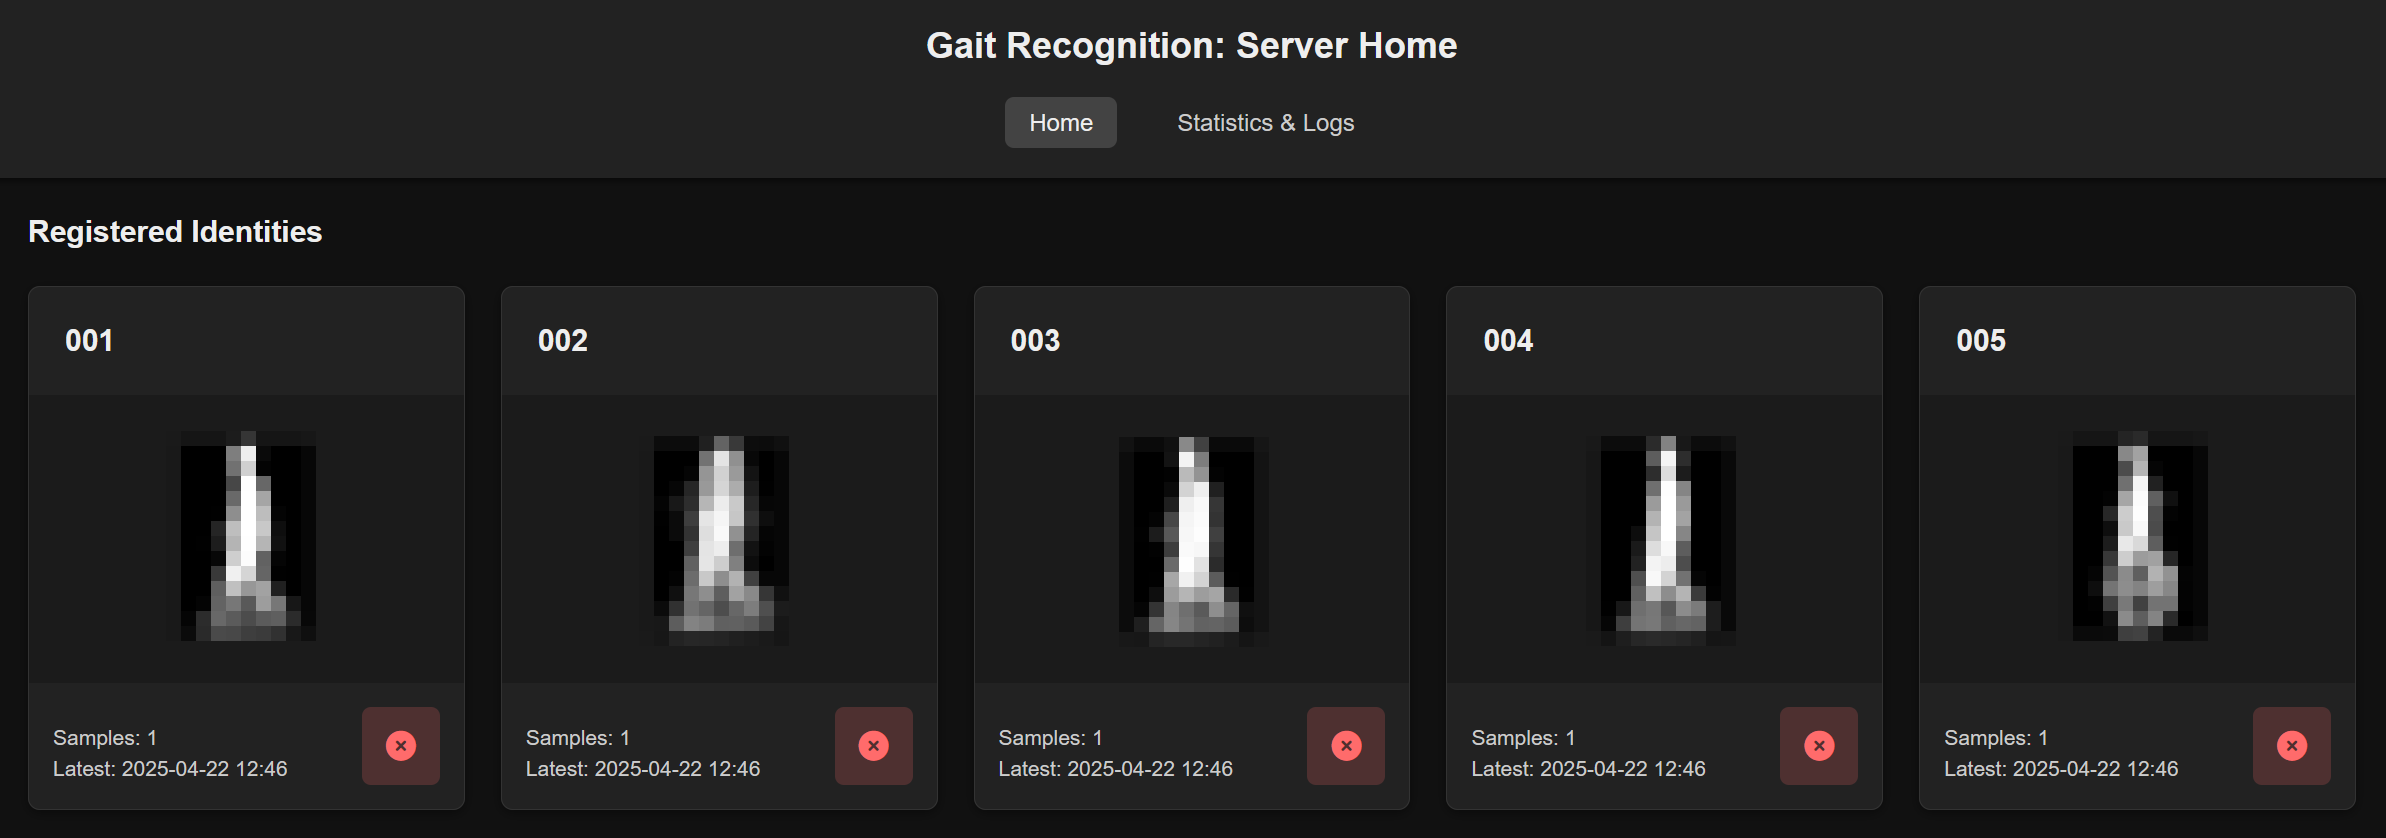
\includegraphics[width=0.8\textwidth]{assets/testing-set-redacted.png}
	\caption{Volunteer Testing Dataset Preview}
	\label{fig:volunteer-testing-set-preview}
\end{figure}

Following this, one of the subjects was instructed to walk through the camera's field of view, with the \ac{acc} application capturing another \ac{gei} sample of the subject.
A few seconds later, the \ac{acc}'s \ac{ui} was updated with the classification result; displaying the subject's anonymised label, the prediction confidence score, and their associated (currently False) access rule --- shown in Figure \ref{fig:identity-classification-known-subject-result} below.

\begin{figure}[H]
	\centering
	
\includegraphics[width=0.8\textwidth]{assets/known-classification-result.png}
	\caption{Identity Classification of Known Subject Result}
	\label{fig:identity-classification-known-subject-result}
\end{figure}

\begin{adjustwidth}{1cm}{}
	\begin{tcolorbox}[colback=green!5, boxrule=0pt, frame empty]
		This result aligns with what was expected for \#FT3, proving that the system is able to correctly classify a known subject.
		The nature of true-positive predictions implies increased accuracy with a larger number of registered samples.
		The accuracy of the system's classification model is evaluated in greater depth in Section \ref{sec:performance-evaluation}.
	\end{tcolorbox}
\end{adjustwidth}

\paragraph{FT4 --- Identity Classification of Unknown Subject}
Following population of the \ac{grs} with the dataset defined in \#FT3, a sixth subject was instructed to walk through the camera's field of view, with the \ac{acc} application producing a \ac{gei} sample of the subject.
The output displayed in the \ac{acc}'s \ac{ui} indicated the predicted identity of this subject was 'Unknown', as expected --- shown in Figure \ref{fig:identity-classification-unknown-subject-result} below.

\begin{figure}[H]
	\centering
	
\includegraphics[width=0.8\textwidth]{assets/unknown-classification-result.png}
	\caption{Identity Classification of Unknown Subject Result}
	\label{fig:identity-classification-unknown-subject-result}
\end{figure}

Checking the back-end console output of the \ac{acc} actually indicated that the subject was misclassified as subject \#003, but with a confidence score of 62.03\% ({"access":false,"confidence":62.03,"person":"003"}).
Because the prediction confidence was below the 75\% threshold defined when implementing the \ac{acc}'s access provision conditions, the \ac{ui} was not updated to display the (incorrect) identity.

\begin{adjustwidth}{1cm}{}
	\begin{tcolorbox}[colback=green!5, boxrule=0pt, frame empty]
		This result aligns with what was expected for \#FT4, with the system correctly dealing with a classification prediction below the set threshold and specifying the subject's identity was unknown.
		This is a critical requirement for security-sensitive applications like \ac{pacs}, as misattribution of identity could result in a security breach.
	\end{tcolorbox}
\end{adjustwidth}

\paragraph{FT5 --- Access Rule Configuration}
From the \ac{grs}' \ac{ui}, a registered identity was selected, loading its 'Identity' page.
The toggle displayed in the top right of the page was then clicked, changing the access rule from 'Disallow' to 'Allow', providing feedback by changing the colour of the toggle from red to green --- shown in Figure \ref{fig:access-rule-configuration} below.

\begin{figure}[H]
	\centering
	\begin{minipage}[t]{0.48\textwidth}
		\centering
		
\includegraphics[width=\textwidth]{assets/toggleoff.png}
		\subcaption{Disallow Status}
	\end{minipage}\hfill
	\begin{minipage}[t]{0.48\textwidth}
		\centering
		
\includegraphics[width=\textwidth]{assets/toggleon.png}
		\subcaption{Allow Status}
	\end{minipage}
	\caption{Access Rule Configuration Toggles}
	\label{fig:access-rule-configuration}
\end{figure}

To confirm the effect of this action, the \ac{grs} database was manually checked, with the 'rule' field in the AccessRule table associated with the identity having been updated to \codeword{1}, representing a True value --- shown in Figure \ref{fig:access-rule-configuration-database} below.

\begin{figure}[H]
	\centering
	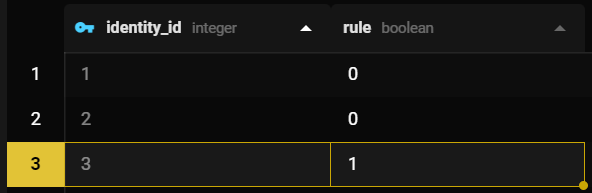
\includegraphics[width=0.7\textwidth]{assets/accessruledbconfig.png}
	\caption{Access Rule Configuration in Database}
	\label{fig:access-rule-configuration-database}
\end{figure}

The steps defined in \#FT3 were then repeated, with the \ac{acc} application now displaying that the (correctly) classified subject was 'Allowed' access, shown in Figure \ref{fig:identity-classification-known-subject-result-access-allowed} below.

\begin{figure}[H]
	\centering
	
\includegraphics[width=0.8\textwidth]{assets/known-classification-result-access-allowed.png}
	\caption{Identity Classification of Known Subject Result with Access Allowed}
	\label{fig:identity-classification-known-subject-result-access-allowed}
\end{figure}

\begin{adjustwidth}{1cm}{}
	\begin{tcolorbox}[colback=green!5, boxrule=0pt, frame empty]
		This result aligns with what was expected for \#FT5, with the system correctly updating the access rule for the identity.
		This demonstrates the end-to-end functionality of \ac{gr} being used as an authentication mechanism for access control.
	\end{tcolorbox}
\end{adjustwidth}

\paragraph{FT6 --- (No) Data Retention}
In line with legislation such as the \ac{gdpr}, it is important that data is not retained for longer than necessary, meaning data used classification and not registration must not be retained by the \ac{acc} or \ac{grs}.

From observing system behaviour, the \ac{acc}' file directory, and \ac{grs} file directory and database, it was found that nothing captured, transmitted, received, or processed during classification operations was ever written to persistent storage.

\begin{adjustwidth}{1cm}{}
	\begin{tcolorbox}[colback=green!5, boxrule=0pt, frame empty]
		This result aligns with what was expected for \#FT6, with the system correctly not retaining data used for classification.
		There is no visual evidence to display for this test, as the requirement is that something not happen.
	\end{tcolorbox}
\end{adjustwidth}

\paragraph{FT7 --- Access Control Atomicity}

Observing the \ac{grs} database, it was found that access rule element in the \ac{acc} \ac{ui} was updated after (and only after) a response to a classification request was received by the \ac{acc} from the \ac{grs}.

\begin{adjustwidth}{1cm}{}
	\begin{tcolorbox}[colback=green!5, boxrule=0pt, frame empty]
		This result aligns with what was expected for \#FT7, with the system only proceeding to access rule provision after a classification result was received.
	\end{tcolorbox}
\end{adjustwidth}

\paragraph{FT8 --- Client's Dependency on the Server}
In a similar fashion to tests \#FT1 and \#FT3, the \ac{acc} was used to submit registration and classification requests while the \ac{grs} was not running.
This resulted in the \ac{acc} displaying an error message stating that an identity could not be registered, or could not be classified respectively --- shown in Figure \ref{fig:client-dependency-on-server} below.

\begin{figure}[H]
	\centering
	\begin{minipage}[t]{0.48\textwidth}
		\centering
		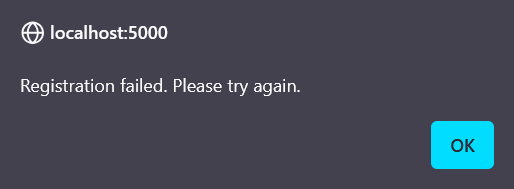
\includegraphics[width=\textwidth]{assets/registrationfail.png}
		\subcaption{Registration Failure}
	\end{minipage}\hfill
	\begin{minipage}[t]{0.48\textwidth}
		\centering
		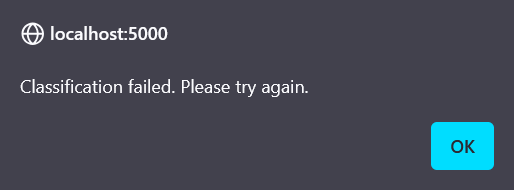
\includegraphics[width=\textwidth]{assets/classificationfail.png}
		\subcaption{Classification Failure}
	\end{minipage}
	\caption{Errors Displayed by the Client if the Server is Not Running}
	\label{fig:client-dependency-on-server}
\end{figure}

\begin{adjustwidth}{1cm}{}
	\begin{tcolorbox}[colback=green!5, boxrule=0pt, frame empty]
		This result aligns with what was expected for \#FT8, with the system correctly not proceeding to access rule provision until a classification result was received.
	\end{tcolorbox}
\end{adjustwidth}

\paragraph{FT9 --- Client Camera Feed and Gait Cycle Previews}
The \ac{acc} was used in tests \#FT1, \#FT3, \#FT6, \#FT7, and \#FT8 to capture and submit \ac{gei} samples to the \ac{grs}.
Throughout these tests, the camera feed and gait cycle previews on the \ac{acc}'s \ac{ui} were displayed and continuously updated as expected.
Figure \ref{fig:camera-feed-and-gait-cycle-previews} below shows a screenshot of the \ac{acc}'s \ac{ui} displaying the camera feed and gait cycle previews during sample capture.

\begin{figure}[H]
	\centering
	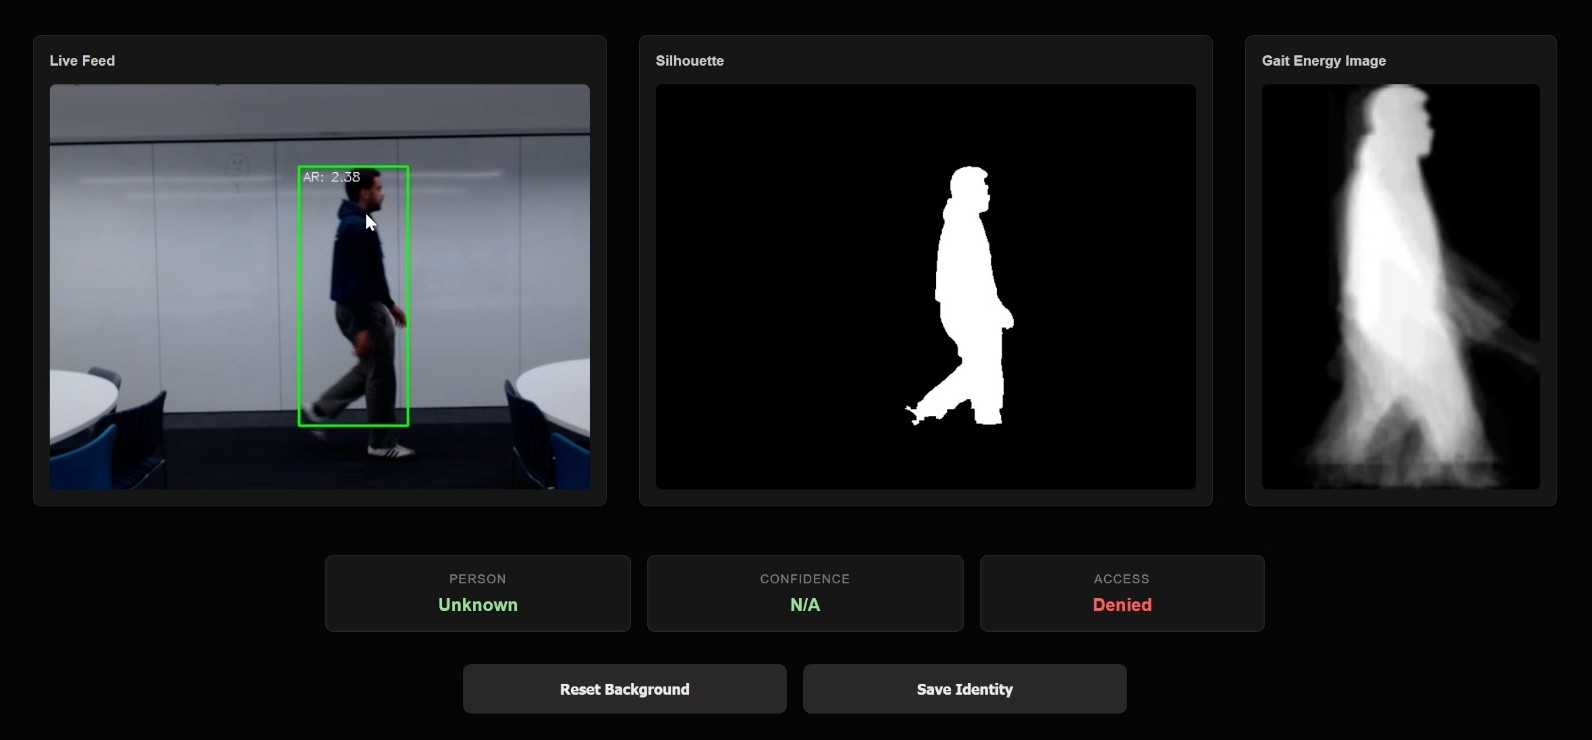
\includegraphics[width=0.8\textwidth]{assets/mid-cycle.jpg}
	\caption{Live Feed, Silhouette, and \ac{gei} Mid-Cycle Previews}
	\label{fig:camera-feed-and-gait-cycle-previews}
\end{figure}

\begin{adjustwidth}{1cm}{}
	\begin{tcolorbox}[colback=green!5, boxrule=0pt, frame empty]
		This result aligns with what was expected for \#FT9, with the system correctly displaying the camera feed and gait cycle previews.
	\end{tcolorbox}
\end{adjustwidth}

\paragraph{FT10 --- Server Activity Logging and Display}
Throughout these tests, when identities were registered, removed, and classified, or when access rules were updated, the \ac{grs}' 'ActivityLog' database tables was updated with log entries as expected.
Figure \ref{fig:server-activity-log-database-entries} below shows a screenshot of the \ac{grs}' 'ActivityLog' database table, listing several log entries relating to tests conducted in this section. 

\begin{figure}[H]
	\centering
	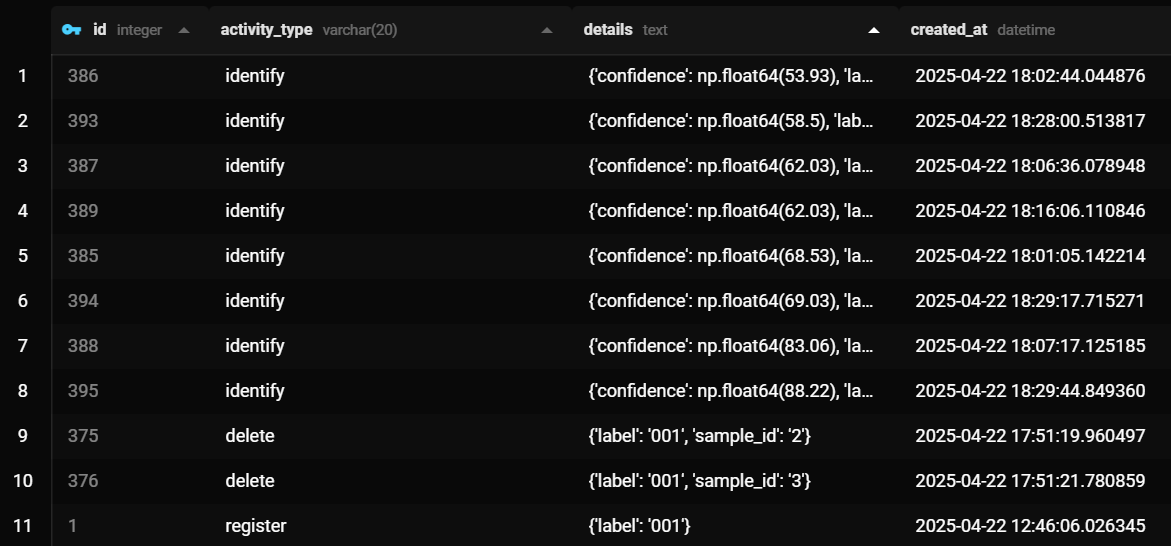
\includegraphics[width=0.6\textwidth]{assets/logentries.png}
	\caption{Server Activity Log Database Entries Example}
	\label{fig:server-activity-log-database-entries}
\end{figure}

Another requirement was for the \ac{grs}' \ac{ui} to display the log entries.
Its 'Statistics \& Logs' page was visited and found to display the logs as expected: in descending creation order --- shown in Figure \ref{fig:server-ui-activity-log-display} below. 

\begin{figure}[H]
	\centering
	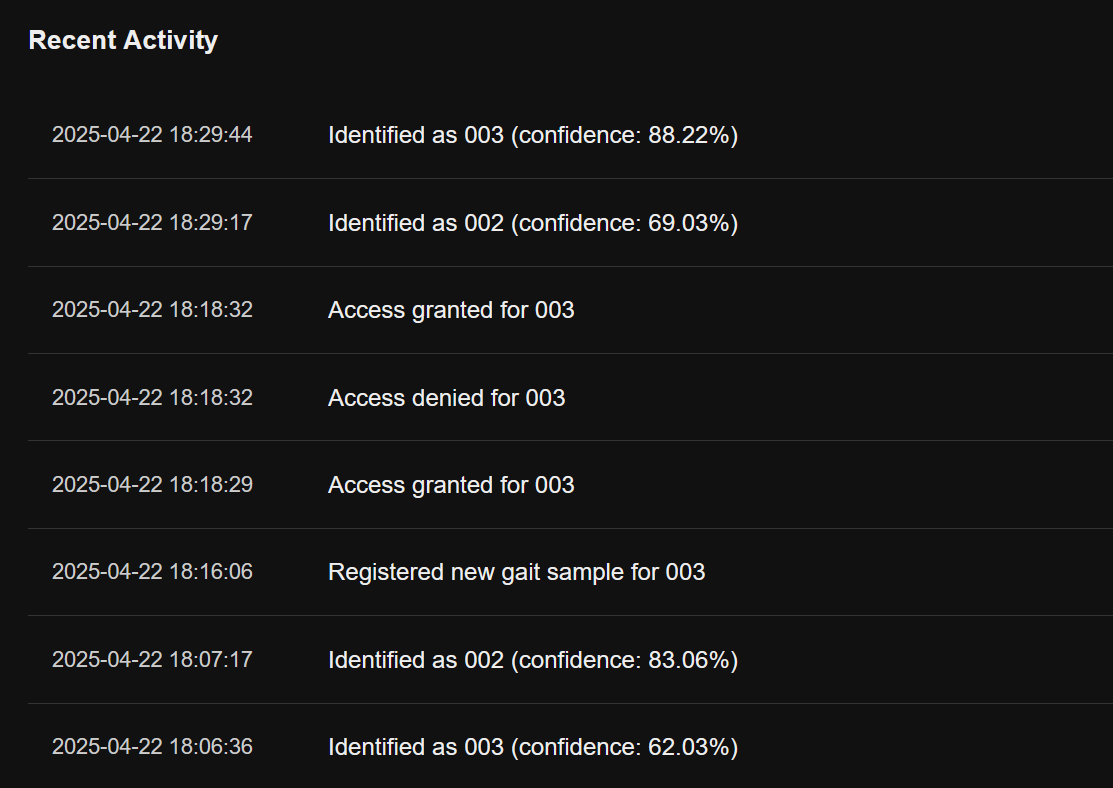
\includegraphics[width=0.6\textwidth]{assets/uilogview.png}
	\caption{Server UI Activity Log Display}
	\label{fig:server-ui-activity-log-display}
\end{figure}

\begin{adjustwidth}{1cm}{}
	\begin{tcolorbox}[colback=green!5, boxrule=0pt, frame empty]
		This result aligns with what was expected for \#FT10, with the system correctly logging and displaying activity.
	\end{tcolorbox}
\end{adjustwidth}

The product of these ten functionality tests shows the \ac{grs} and \ac{acc} meet expected functionality as defined in Section \ref{subsec:functionality-testing-plan}, demonstrating how \ac{gr} can be used as an authentication mechanism for access control.
